\documentclass[submission, copyright, creativecommons]{eptcs}
\providecommand{\event}{TERMGRAPH 2022} % Name of the event you are submitting to
% \usepackage{breakurl}             % Not needed if you use pdflatex only.
\usepackage{underscore}           % Only needed if you use pdflatex.

% My packages
\usepackage{orcidlink} % Orcid links
\newcommand\Mark[1]{\textsuperscript#1}

\usepackage{subcaption} % Side by side figures
\usepackage{amssymb} % \square command
% Footnotes inside tables
\usepackage{footnote}
\usepackage{csquotes} % enquote command
\usepackage{glossaries} % Glossary
\usepackage{threeparttable} % Tables with notes
\makesavenoteenv{tabular}
\makesavenoteenv{table}
\usepackage[nameinlink]{cleveref} % Reference footnotes.
\crefname{figure}{{figure}}{figures}
\Crefname{figure}{{Figure}}{Figures}
\crefformat{footnote}{#2\footnotemark[#1]#3}
% Math
\newtheorem{definition}{Definition}
\newcommand{\definitionautorefname}{Definition}
% Acronyms
\newacronym{bpmn}{BPMN}{Business Process Modeling Notation}

\title{Formalization and analysis of BPMN using graph transformation systems}
\author{Tim Kräuter\Mark{*}\orcidlink{0000-0003-1795-0611}, \quad
Harald König\Mark{\textdagger}\Mark{*}\orcidlink{0000-0001-6304-6311}, \quad
Adrian Rutle\Mark{*}\orcidlink{0000-0002-4158-1644}, \quad
Yngve Lamo\Mark{*}\orcidlink{0000-0001-9196-1779}
\institute{
\Mark{*}Western Norway University of Applied Sciences, Bergen, Norway
}
\institute{
\Mark{\textdagger}University of Applied Sciences, FHDW, Hannover, Germany}
\email{tkra@hvl.no, harald.koenig@fhdw.de, aru@hvl.no, yla@hvl.no}
}
\def\titlerunning{Formalization and analysis of BPMN using graph transformation systems}
\def\authorrunning{Kräuter \textit{et al.}}
\begin{document}
\maketitle

% Maximum 8 pages for the first extended abstract(including references)!
% Maximum of 10 pages for the first revision.

\begin{abstract}
The BPMN is a widely used standard notation for defining intra- and inter-organizational workflows.
However, the informal description of the BPMN execution semantics leads to different interpretations of BPMN constructs and difficulties in checking behavioral properties.
In this paper, we propose a formalization of the execution semantics of BPMN that, compared to other approaches, covers most of the BPMN constructs.
Our approach is based on a model transformation from BPMN models to graph transformation systems.
As proof of concept, we have implemented our approach in an open-source web-based tool.
\end{abstract}

\section{Introduction}
% Short Motivation: Formalization of the natural language semantics and model checking
\gls*{bpmn} \cite{objectmanagementgroupBusinessProcessModel2013} is a widely used standard notation to define intra- and inter-organizational workflows.
However, the informal description of the BPMN execution semantics leads to different interpretations of BPMN constructs and difficulties in checking behavioral properties \cite{corradiniFormalApproachAnalysis2021}.
To this end, we propose a formalization that, compared to other approaches, covers most of the BPMN constructs.

%Our approach is depicted as a BPMN process model in \cref{fig:approach}.
Our approach is based on a model transformation from BPMN process models to graph transformation systems using rule generation templates.
Thus, our approach constructs a new graph transformation system, i.e., graph transformation rules and a start graph for each BPMN process model.
This is a significant difference compared to other approaches, such as \cite{corradiniFormalApproachAnalysis2021, vangorpVisualTokenbasedFormalization2013}, where only the BPMN process model is parsed, but the rewrite rules are fixed.
Generating specific rules for each model leads to possibly more but simpler transformation rules that can be matched faster.
Essentially, complexity is partly shifted from the transformation rules to their generation.
The generated rules are tailored to a given process model and thus are simpler than the general rules in \cite{vangorpVisualTokenbasedFormalization2013}.

%TODO Move this down to later and explain all ingredients in let us say a discussion or summary or section
\begin{figure}[h]
    \centering
    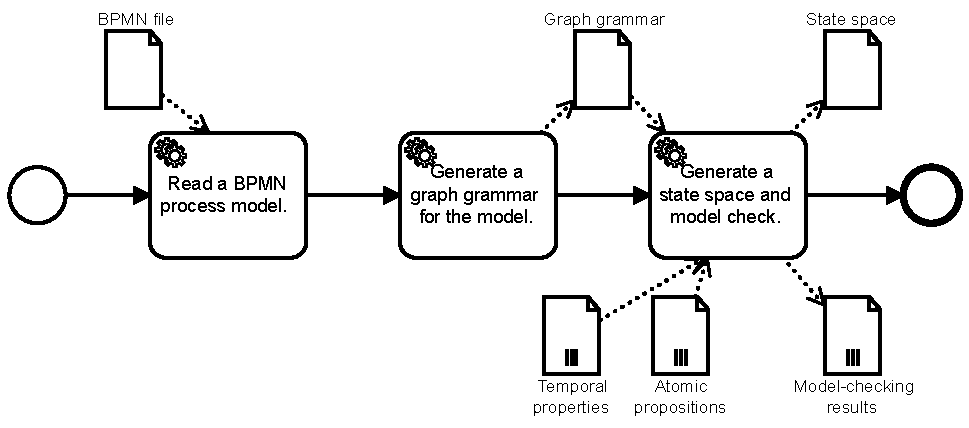
\includegraphics[width=0.8\textwidth]{images/full-approach.pdf}
    \caption{Overview of the proposed approach}
    \label{fig:approach}
\end{figure}

% Paper outline
The remainder of this paper is structured as follows.
First, we describe the semantics formalization using graph transformation systems (\cref{sec:formalization}) before explaining how this can be utilized for model checking BPMN-specific and custom properties (\cref{sec:modelChecking}).
Then, we shortly present the web-based tool implementing our approach.
Finally, we discuss related work regarding BPMN construct coverage in \cref{sec:relatedWork} and conclude in \cref{sec:conclusion}.

\section{Preliminaries}
% Describe the application are
In this paper, we apply graph rewriting theory to formalize the execution semantics of BPMN.
Thus, in this section, we will briefly introduce BPMN and its execution semantics.
Please refer to \cite{freundRealLifeBPMNUsing2019} or the BPMN specification \cite{objectmanagementgroupBusinessProcessModel2013} for further information about BPMN.
% Describe the applied theory.
Furthermore, we describe the theoretical background behind our application of graph rewriting.
\subsection{BPMN}
% Introduce BPMN
BPMN  is a widely used standard notation to define intra- and inter-organizational workflows.
\Cref{fig:bpmnMetamodel} depicts the structure of BPMN process models and the corresponding BPMN symbols contained in clouds.

\begin{figure}[h]
  \centering
  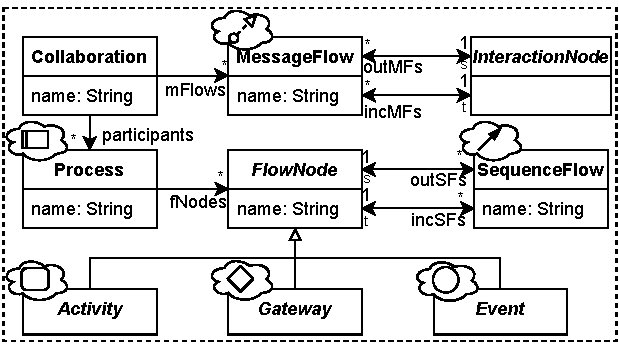
\includegraphics[width=0.75\linewidth]{images/bpmn_semantics-bpmn-metamodel.pdf}
  \caption{Simplified excerpt of the BPMN metamodel \cite{objectmanagementgroupBusinessProcessModel2013}}
  \label{fig:bpmnMetamodel}
\end{figure}

A BPMN process model is represented by a \textsf{Collaboration} that has \textsf{participants} and \textsf{MessageFlows} between \textsf{InteractionNodes} (see  \cref{fig:bpmnMetamodel}).
Each participant is a \textsf{Process} containing \textsf{FlowNodes} connected by \textsf{SequenceFlows}.
A \textsf{FlowNode} is either an \textsf{Activity}, \textsf{Gateway}, or \textsf{Event}.
Many types of \textsf{Activities}, \textsf{Gateways}, and \textsf{Events} exist, such as start and end events which are used in \cref{fig:approach}.
Activities represent certain tasks to be carried out during a process, while events may happen during the execution of these tasks.
Furthermore, gateways model conditions, parallelizations and synchronizations \cite{freundRealLifeBPMNUsing2019}.

% BPMN semantics: Token distribution
The BPMN execution semantics are described using the concept of \emph{tokens} \cite{objectmanagementgroupBusinessProcessModel2013}.
BPMN process models are executed by triggering one or more of their start events, leading to the creation of a token at each triggered start event.
Tokens are transported between flow nodes by sequence flows (arrows)
\footnote{The visual bpmn-js token simulation available at \url{https://bpmn-io.github.io/bpmn-js-token-simulation/modeler.html} greatly helps to understand BPMN execution semantics.}.
% Activities
Activities can start when at least one token is located on an incoming sequence flow.
The start of an activity will move the incoming token to the activity.
When an activity finishes, it will create one token at each outgoing sequence flow.
% Gateways
Different gateway types exist, for example, for parallelization, synchronization, XOR and OR distribution of tokens.
% Events (basic)
Events consume and create tokens similar to activities but have additional semantics depending on their type.
For example, message events will create or consume messages.

\subsection{Theoretical background}
We use typed attributed graphs for the formalization of the BPMN execution semantics.
Each state, i.e., token distribution during the execution of a BPMN model, is represented as an attributed graph typed by the BPMN execution type graph which is introduced in \cref{sec:formalization}.

% Groove uses the single pushout approach with negative application conditions.
Regarding graph transformation, we utilize the single-pushout (SPO) approach with negative application conditions (NAC) \cite{ehrigALGEBRAICAPPROACHESGRAPH1997}.
In addition, we utilize \emph{nested rules} with quantification to make parts of a rule applied repeatedly or optionally \cite{rensinkNestedQuantificationGraph2006,rensinkHowMuchAre2017}.
%SPO is sufficient to formalize the BPMN execution semantics, and the automatic removal of dangling edges is not a problem since .
Moreover, we utilize NACs to implement more intricate parts in the BPMN execution semantics, such as the termination of processes. 
In SPO rewriting, a graph transformation rule is defined as a partial graph morphism $L \to R$, where in our case, $L$ and $R$ are typed attributed graphs. 



\section{BPMN semantics formalization} \label{sec:formalization}

Since our approach is based on a model transformation from BPMN to graph transformation systems, we generate a \emph{start graph} and \emph{graph transformation rules} for a given BPMN process model.
The approach supports the BPMN constructs depicted in \cref{fig:bpmnConstructsOverview}.

\begin{figure}[h]
    \centering
    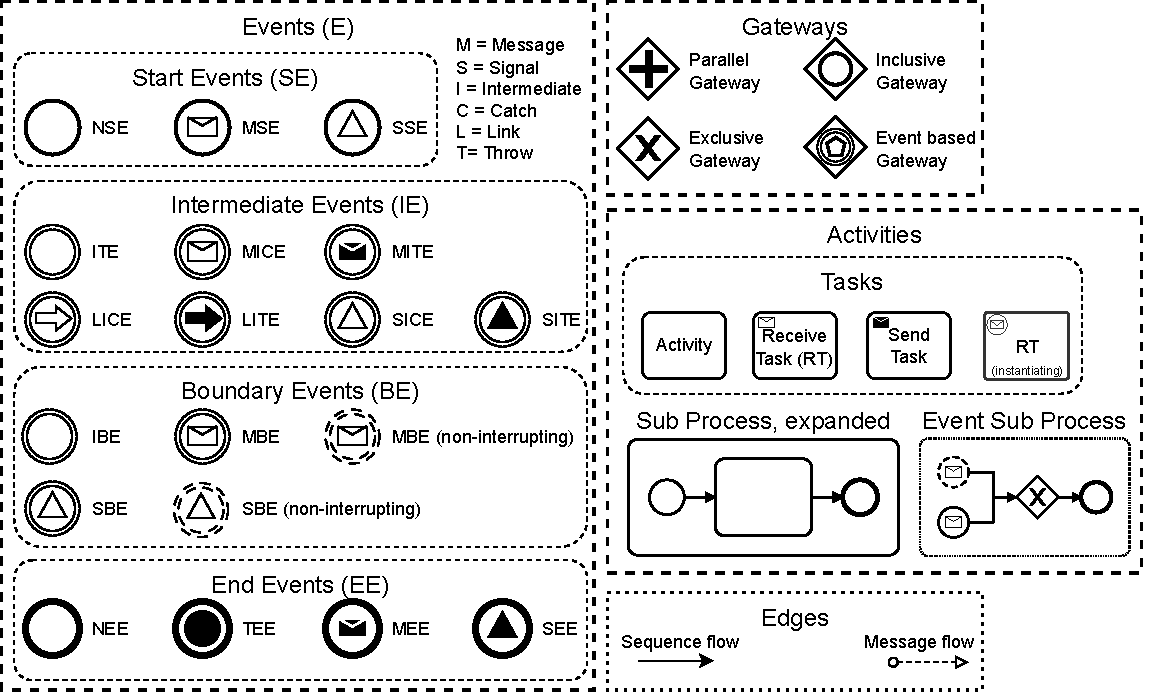
\includegraphics[width=0.99\textwidth]{images/bpmn_semantics-feature-overview.pdf}
    \caption{Overview of the supported BPMN constructs (structure adapted from \cite{houhouFirstOrderLogicVerification2022})}
    \label{fig:bpmnConstructsOverview}
\end{figure}

Our formalization of BPMN is token-based, as in the informal description of the BPMN specification \cite{objectmanagementgroupBusinessProcessModel2013}.
Thus, to describe processes holding tokens during execution, we use the type graph shown in \cref{fig:typeGraph}.
The type graph is depicted using a UML class diagram-like syntax.

\begin{figure}
  \centering
  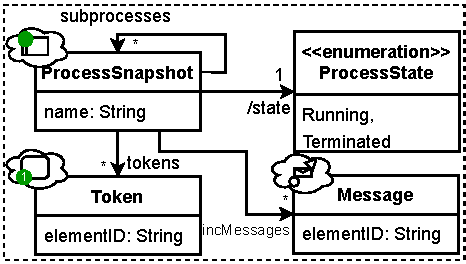
\includegraphics[width=0.5\linewidth]{images/bpmn_semantics-typegraph.pdf}
  \caption{BPMN execution type graph}
  \label{fig:typeGraph}
\end{figure}

We use \textsf{ProcessSnapshot} to denote a running BPMN process with a specific token distribution that describes one state in the history of process states during the execution.
Every \textsf{ProcessSnapshot} has a set of \textsf{tokens}, incoming \textsf{messages}, and \textsf{subprocesses}.
A \textsf{ProcessSnapshot} has the state \textsf{Terminated} if it has no \textsf{tokens} or \textsf{subprocesses}.
Otherwise, it has the state \textsf{Running}.
A \textsf{Token} has an \textsf{elementID}, which points to the BPMN \textsf{Activity} or the \textsf{SequenceFlow} at which it is located.
A \textsf{Message} has an \textsf{elementID} pointing to a \textsf{MessageFlow}.
To concisely depict graphs conforming to this type graph, we introduce a concrete syntax in the clouds attached to the elements.
%It extends the BPMN syntax by adding tokens.
Tokens are represented as colored circles drawn at their specified positions in a model.
In addition, we use colored circles at the top left of the bounding box which represents instances of the BMPN \textsf{Process}; these circles represent process snapshots.
The color of the token must match the color of the process snapshot holding the token.
The concrete syntax was inspired by the bpmn-js-token-simulation\footnote{\url{https://github.com/bpmn-io/bpmn-js-token-simulation}}.
Using this type graph, we can now define how the start graph and graph-transformation rules for the different BPMN constructs are created.

% How is a start graph generated?
The generation of the start graph for a BPMN model is straightforward.
For each process in the BPMN model, we generate a process snapshot if the process contains a none start event (NSE).
Then, for each NSE, we add a token to the respective process snapshot.
An example of a start graph is shown in \cref{fig:startGraph} using abstract and concrete syntax.
Furthermore, we consider allowing the user to define a start graph similar to how he can define atomic propositions for custom properties (see \cref{subsec:customProperties}).

\begin{figure}[h]
    \centering
    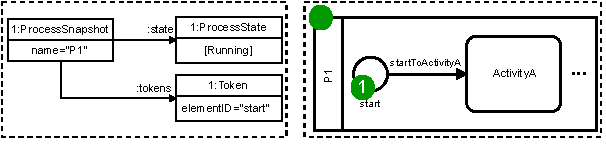
\includegraphics[width=0.7\textwidth]{images/startGraph.pdf}
    \caption{Example start graph in abstract (left) and concrete syntax (right)}
    \label{fig:startGraph}
\end{figure}

The model transformation generates one or more graph transformation rules for each \textsf{FlowNode} in a BPMN model.
To give an intuition about the model transformation, we will first describe example results, i.e., generated rules for a NSE, a task, and a send/receive message event.
Afterward, we will explain how these---and other---rules are created by our model transformation.

\Cref{fig:gtRuleAbstract} depicts an example graph transformation rule ($L \to R$) for a NSE in abstract syntax.
The rule is straightforward and moves a token from the start event to its outgoing sequence flow.
For the rest of the paper, we will depict all rules in the concrete syntax introduced earlier.
The rule from \cref{fig:gtRuleAbstract} depicted in concrete syntax is shown in \cref{fig:gtRuleConcrete}.


\begin{figure}[h]
    \centering
  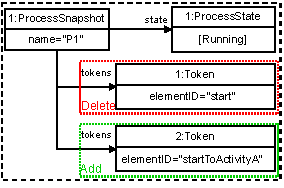
\includegraphics[width=0.8\textwidth]{images/rule_abstract.pdf}
  \caption{Example graph transformation rule for a NSE (abstract syntax)}  \label{fig:gtRuleAbstract}
\end{figure}

\begin{figure}[h]
    \centering
  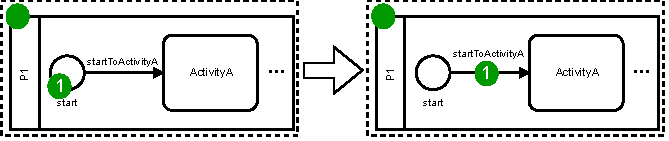
\includegraphics[width=0.6\textwidth]{images/rule_concrete.pdf}
  \caption{Example graph transformation rule for a NSE (concrete syntax)}
  \label{fig:gtRuleConcrete}
\end{figure}

The rule in \cref{fig:taskRules} represents the start of a task, which will move one token from the incoming sequence flow to the task itself.

\begin{figure}[h]
    \centering
    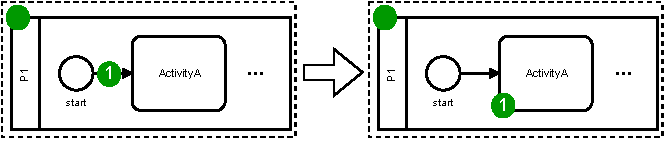
\includegraphics[width=0.6\textwidth]{images/bpmn_semantics-rules.pdf}
    \caption{Example graph transformation rule to start a task.}
    \label{fig:taskRules}
\end{figure}

The left rule in \cref{fig:messageEventRules} realizes a message throw event, and the right rule implements a message catch event.
The message catch event rule consumes a token and a message and creates an outgoing token.
The message throw event rule moves the token through the event and may send a message to a waiting process snapshot if it has a token waiting at the corresponding message receive event.
An optional existential quantifier is used to send a message only if the receiving process is ready to receive it.
The message throw (catch) rule generation is realized by the rule generation template given in \autoref{fig:throwEventTemplates} (\autoref{fig:catchMessageTemplates}) later.

\begin{figure}[h]
    \centering
    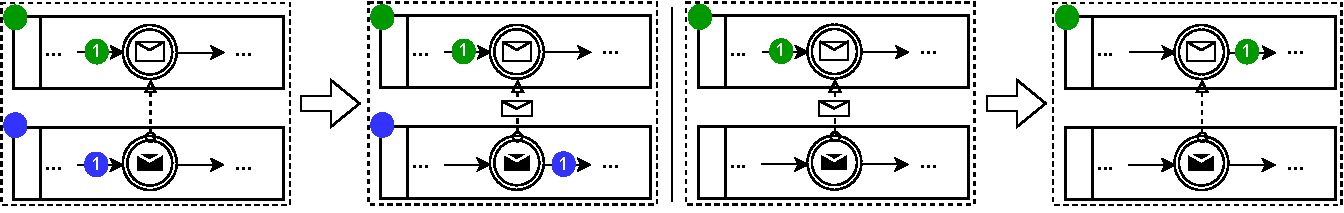
\includegraphics[width=1\textwidth]{images/bpmn_semantics-message-events.pdf}
    \caption{Rules for message intermediate throw events (left) and catch events (right)}
    \label{fig:messageEventRules}
\end{figure}

To summarize, we described four example rules and introduced a concrete syntax to depict them concisely and understandably.
In the following subsections, we use this concrete syntax to describe how these rules and rules for other flow nodes are generated by our model transformation.
Elements of the model transformation are depicted using rule generation templates that describe how specific rules are created for various flow nodes.
We explain rule generation for (i) process instantiation and termination, (ii) activities and subprocesses, (iii) gateways, as well as (iv) message events.
%ADD


\subsection{Process instantiation and termination} \label{subsec:instAndTermination}

\autoref{fig:startAndEndTemplate} depicts the rule generation templates for start and end events.
All rule generation templates show a BPMN structure defined in the left column and the applicable rule generation template in the right column.
The structures in the left column show instances of the BPMN metamodel (\autoref{fig:bpmnMetamodel}) and the ones in the right column show the rules which are typed by the BPMN execution type graph (see \autoref{fig:typeGraph}.
All the rule generation templates can be found in \cite{timkrauterArtifactsTERMGRAPH2022}.


\begin{figure}[h]
    \centering
    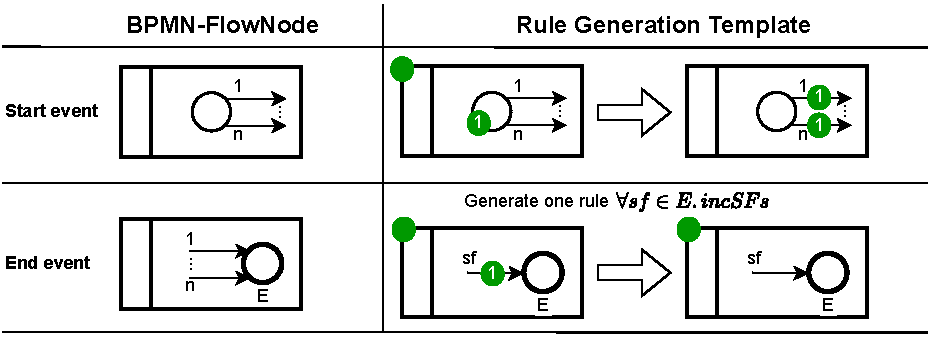
\includegraphics[width=.9\textwidth]{images/start_end_template.pdf}
    \caption{Rule generation templates for start and end events}
    \label{fig:startAndEndTemplate}
\end{figure}

% Start Event + Refer to the start graph.
The start event rule in \autoref{fig:gtRuleConcrete} is generated by the start event rule template.
The tokens located on the start events are deleted by start event rules, while one token for each outgoing sequence flow is added.
If a start event has more than one outgoing sequence flow, it functions as an \textit{implicit parallel gateway}, forking the control flow by creating one token for each of the sequence flows (see parallel gateway in \autoref{fig:gatewayTemplates}).
Initially, the tokens on the start events are given by the start graph of the graph transformation system (see e.g. \autoref{fig:startGraph}).
    
% End Event
The generated end event rules delete tokens one by one for each incoming sequence flow.
However, they do not terminate processes.
% General termination rule
Process termination is implemented with a generic rule---independent of the input BPMN model---which is applicable to all process snapshots.
The rule is automatically generated once during the model transformation.
It is used to terminate processes and subprocesses if they do not have any tokens.
The rule uses negative-application conditions to only change the state of the process snapshot from running to terminated if it has no tokens and subprocesses.
The concrete termination rule in Groove is given as an artifact \cite{timkrauterArtifactsTERMGRAPH2022}.

% Receive tasks instantiation (low priority)
% Exclusive event-based gateway instantiation (low priority)
\subsection{Activities \& Subprocesses}
% Normal activities

\autoref{fig:activityTemplates} depicts the rule generation templates for activities and subprocesses.
Activity execution is divided into two steps implemented by two rule templates.
The upper template generates one rule for each incoming sequence flow to start the activity.
An activity can be started using a token positioned at any of its incoming sequence flows.
Thus, multiple incoming sequence flows represent an \textit{implicit exclusive gateway} (see exclusive gateway in \autoref{fig:gatewayTemplates}).
The sample rule in \autoref{fig:taskRules} is generated by this rule template.

The bottom rule template generates one rule that ends the activity.
It deletes a token at the activity and adds one token at each outgoing sequence flow.
Similar to start events, this implicitly encodes the same forking behavior as a parallel gateway (see \autoref{fig:gatewayTemplates}). 

\begin{figure}[h]
    \centering
    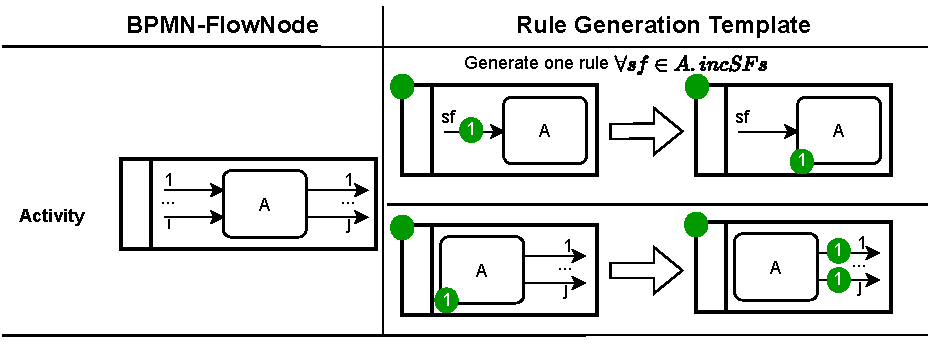
\includegraphics[width=1\textwidth]{images/activities_template.pdf}
    \caption{Rule generation template for activities and subprocesses}
    \label{fig:activityTemplates}
\end{figure}

% Subprocesses/Call activities
Subprocess execution is similar to activity execution.
The upper template generates one rule for each incoming sequence flow.
The rule deletes an incoming token and adds a process snapshot representing a subprocess. 
The addition of this process snapshot is represented with a colored circle on the top left corner of the subprocess with a token at each of its start events.
To depict the \textsf{subprocesses} relation in \autoref{fig:typeGraph}, we chose the same color for the outer ring of the subprocess snapshot and its tokens.
If the subprocess has no start events, a token for every activity and gateway without incoming sequence flows is created. %, as defined in the BPMN specification.

The bottom rule template generates one rule to delete a terminated process snapshot and adds tokens at each outgoing sequence flow.
Subprocesses are terminated by a generic rule (see section \ref{subsec:instAndTermination}) if they neither have tokens nor subprocesses.


% Send/Receive tasks (mentioned/shown with message events later)
\subsection{Gateways}
\autoref{fig:gatewayTemplates} depicts the rule generation templates for parallel and exclusive gateways.
% Parallel
A parallel gateway can synchronize incoming sequence flows and fork outgoing sequence flows simultaneously.
Thus, one rule is generated that deletes one token from each incoming sequence flow and adds one token to each outgoing sequence flow.

\begin{figure}[h]
    \centering
    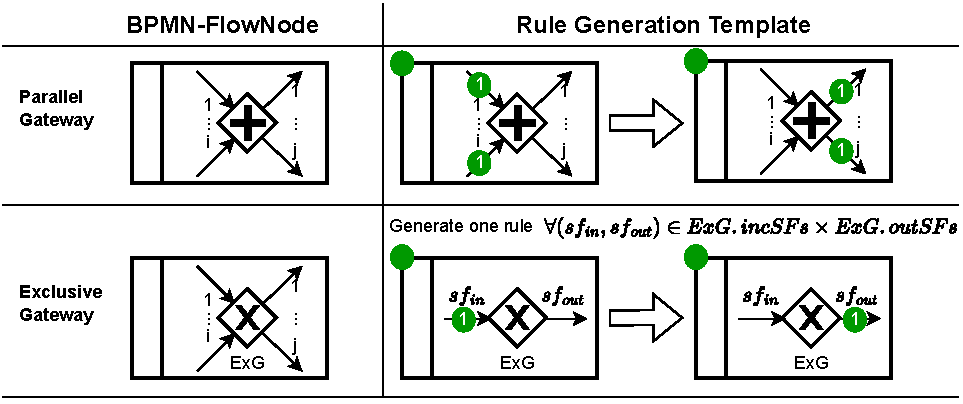
\includegraphics[width=1\textwidth]{images/gateways_template.pdf}
    \caption{Rule generation template for gateways}
    \label{fig:gatewayTemplates}
\end{figure}

% Exclusive --> Exception no incoming flows in sub-processes (token taken from gateway directly)
Exclusive Gateways are triggered by exactly one incoming sequence flow, and exactly one outgoing sequence flow is triggered.
Thus, one rule must be generated for every combination of incoming and outgoing sequence flows.
However, the resulting rule is simple since it only deletes a token from an incoming sequence flow and adds a token to an outgoing sequence flow.

% Event-based with different event combinations
% Mention unsupported types?
\subsection{Message Events}
% Message throw
\autoref{fig:throwEventTemplates} depicts the rule generation templates for \textit{message intermediate throw events} (\textsf{MITE} in \autoref{fig:bpmnConstructsOverview}).
% Message throw with intermediate catch message events
The upper rule describes how message throw events interact with message intermediate catch events.
A \textit{message throw event} consumes an incoming token and adds a token at each outgoing sequence flow.
In addition, it sends one message to each waiting process by adding it to the incoming messages of the process.
However, sending each message is optional, meaning that if a process is not ready to consume a message immediately, the message is not created.
%This behavior corresponds to the BPMN semantics \cite{objectmanagementgroupBusinessProcessModel2013}.
We implement optional message sending using a nested rule with quantification.
Concretely, we use an optional existential quantifier to send a message only if the receiving process runs and is ready to receive it \cite{rensinkNestedQuantificationGraph2006}.

\begin{figure}[h]
    \centering
    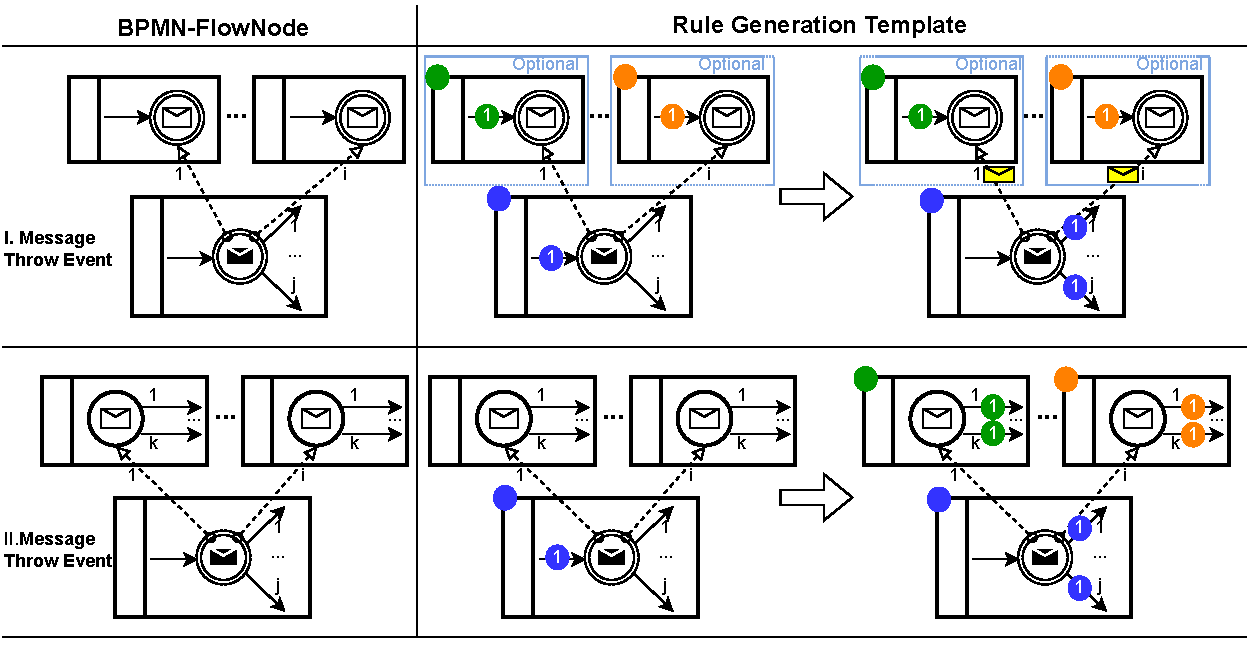
\includegraphics[width=1\textwidth]{images/throw_messages.pdf}
    \caption{Rule generation template for message throw events}
    \label{fig:throwEventTemplates}
\end{figure}

% Message throw with message start events
The bottom rule shows how message intermediate throw events trigger new process instances when interacting with message start events.
For each receiving message start event, a new process snapshot with one token at each outgoing sequence flow is created.
It is worth noting that a message throw event might interact with message intermediate catch events and message start events \textit{simultaneously}.
Thus, the rule generation templates in \autoref{fig:throwEventTemplates} can be mixed, i.e., messages can be sent and processes instantiated by one message throw event.
We only separated message throw behavior into two rule templates for presentation purposes.
% Explain the similarity to Send-tasks.
Furthermore, \textit{message end events} and \textit{send task}s behave similarly regarding message creation and process instantiation.
%However, a \textit{Send Task} executes the message behavior when ending the task, while both send tasks and message end evens change tokens according to their respective rule templates (see \autoref{fig:startAndEndTemplate} and \autoref{fig:activityTemplates}).
% Explain currently, only one incoming sequence flow is allowed (not done).

% Message catch + Receive Task
\autoref{fig:catchMessageTemplates} depicts the rule generation templates for \textit{message intermediate catch event}s and \textit{receive task}s.
To trigger a message intermediate catch event or a receive task, only one message at an incoming message flow is needed.
Thus, one rule is generated for each incoming message flow.
The upper rule template shows that message intermediate catch events delete one message and one token, and, add a token at each outgoing sequence flow.
In the bottom rule template, one can see that \textit{receive task} rules are similar to the \textit{activity} rules in \autoref{fig:activityTemplates}, but they also delete a message when a \textit{receive task} is started.

\begin{figure}[h]
    \centering
    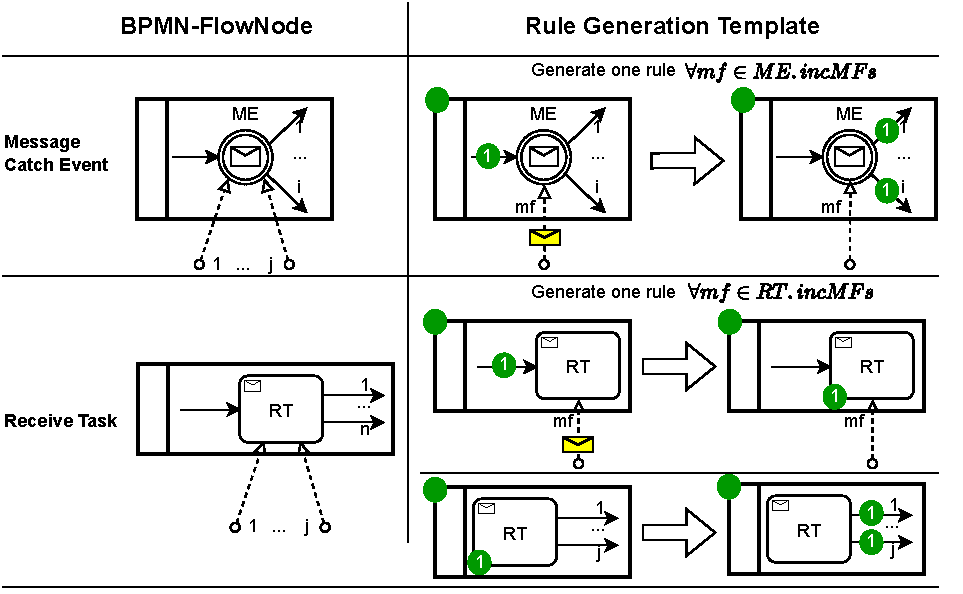
\includegraphics[width=1\textwidth]{images/catch_messages.pdf}
    \caption{Rule generation template for message catch events and receive tasks}
    \label{fig:catchMessageTemplates}
\end{figure}

% Link (maybe if space)

% Not enough space for:
% Signal
% Terminate end
% Boundary events
% Event subprocesses?

\section{Model checking BPMN} \label{sec:modelChecking}

Model checking a BPMN process model is possible using the generated graph transformation system.
Besides a graph transformation system, a set of temporal properties to be checked and the atomic propositions used in these properties must be supplied (see \cref{fig:approach}).
An atomic proposition can be formalized as a graph and holds in a given state if there exists a match from the underlying graph of the proposition to the graph representing the state.
This enables model checking of temporal properties, for example, LTL properties, using the defined atomic propositions.

We differentiate between \emph{BPMN-specific properties} defined for all BPMN process models and \emph{custom properties} tailored towards a particular BPMN process model.
We do not consider structural properties (like conformance to the syntax of PBMN) since they can be checked using a standard process modeling tool without implementing execution semantics.
We will now give an example of two predefined BPMN-specific properties and show how they can be checked using our approach.
Then, we describe how custom properties can be constructed and checked.

\subsection{BPMN-specific properties}
\textit{Safeness} and \textit{Soundness} properties are defined for BPMN in \cite{corradiniClassificationBPMNCollaborations2018}.
A BPMN process model is \emph{safe} if, during its execution, at most one token occurs along the same sequence flow \cite{corradiniClassificationBPMNCollaborations2018}.
Soundness is further decomposed into (i) \emph{Option to complete}: any running process instance must eventually complete, (ii) \emph{Proper completion}: at the moment of completion, each token of the process instance must be in a different end event, as well as (iii) \emph{No dead activities}: any activity can be executed in at least one process instance \cite{corradiniClassificationBPMNCollaborations2018}.
As an example, we will now describe how to implement the \emph{Safeness} and \emph{Option to complete} properties.

% Safeness
\textbf{Safeness} is checked using the LTL property defined in \eqref{eq:safeness}.
The atomic property \textsf{Unsafe} is true if two tokens of one process snapshot point to the same sequence flow. This atomic proposition \textit{Unsafe} is depicted in \autoref{fig:unsafe}; Groove rules for all the atomic proposition are included in \cite{timkrauterArtifactsTERMGRAPH2022}.
% Option to complete
\emph{Option to complete} is checked using the LTL property defined in \eqref{eq:optionToComplete}.
The atomic proposition \textsf{AllTerminated} is true if there exists no process snapshot in the state \textsf{Running}, i.e., all process snapshots are \textsf{Terminated}\cref{footnote:atomicProps}.

\noindent\begin{minipage}{.5\linewidth}
\begin{equation} \label{eq:safeness}
  \square (\neg \,\text{Unsafe})
\end{equation}
\end{minipage}%
\begin{minipage}{.5\linewidth}
\begin{equation} \label{eq:optionToComplete}
  \lozenge ( \square(\text{AllTerminated})) 
\end{equation}
\end{minipage}
\vskip.3\baselineskip

Both properties can be checked using our implementation \cite{timkrauterArtifactsTERMGRAPH2022}.
To fully check Soundness, we need to check \textit{Proper Completion} and \textit{No Dead Activities}.
The information needed to check these properties is present in the generated state space.

\subsection{Custom properties} \label{subsec:customProperties}
% Defining atomic propositions in BPMN is a novelty.
To make model checking user-friendly, we envision users defining atomic propositions in the extended BPMN syntax, i.e., the concrete syntax introduced in \autoref{fig:typeGraph}.
Thus, to define an atomic proposition, we let the user attach tokens to a BPMN process snapshots, which we can automatically convert to a graph representing an atomic proposition.

For example, the token distribution shown in \cref{fig:atomicProposition} defines two running process snapshots with a token in task A.
Differently colored tokens define different process snapshots.
A user could use this property, for example, to check if, eventually, two processes are executing task A simultaneously.
Thus, a user does not need to be aware of the graph transformation semantics used for execution, which is a significant advantage compared to other approaches.

\begin{figure}[h]
    \centering
    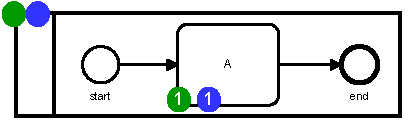
\includegraphics[width=0.45\textwidth]{images/bpmn_semantics-atomic-proposition.pdf}
    \caption{Token distribution defining an atomic proposition.}
    \label{fig:atomicProposition}
\end{figure}

\section{Implementation} \label{sec:impl}
% Tool

\begin{figure}[h]
    \centering
    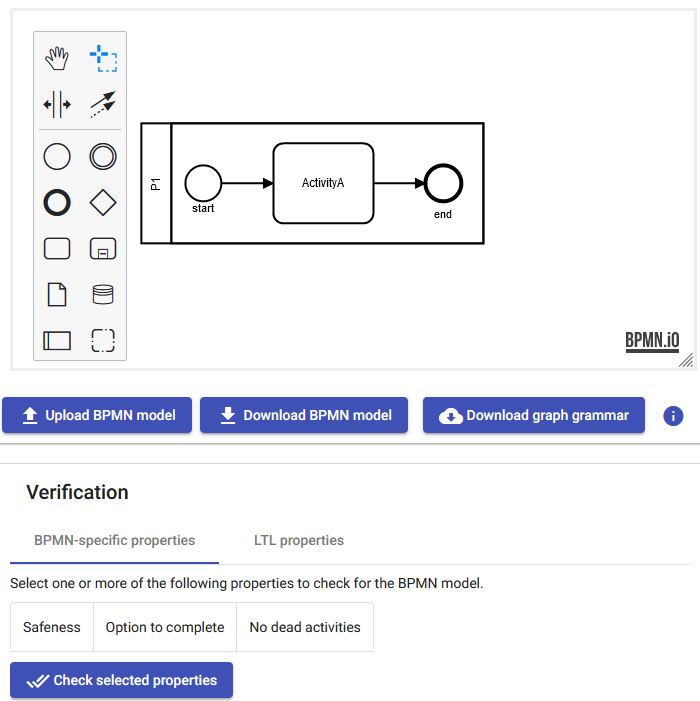
\includegraphics[width=0.7\textwidth]{images/impl.png}
    \caption{Screenshot of the tool}
    \label{fig:implScreenshot}
\end{figure}

\Cref{fig:implScreenshot} depicts a screenshot of the implemented tool.
The tool is open-source, publicly available, and does not require any installation \cite{timkrauterArtifactsTERMGRAPH2022}.
The first two steps of our approach, i.e., reading and transforming BPMN models to graph transformation systems, are implemented and usable through the web-based tool.
Then one can use the graph-transformation tool Groove\footnote{\url{https://groove.ewi.utwente.nl/about}} for state space generation and model checking locally.
We are currently working on extending our tool such that model-checking can be done without installing Groove locally.
Groove implements SPO with NACs and thus has all the features we need.
% Evaluation
To evaluate the correctness of our implementation, we created a comprehensive test suite, which demonstrates correct rule generation for the implemented BPMN constructs \cite{timkrauterArtifactsTERMGRAPH2022}.

\section{Related work} \label{sec:relatedWork}
% Van gorp
A BPMN formalization based on in-place graph transformation rules is given in \cite{vangorpVisualTokenbasedFormalization2013}.
The formalization covers a substantial part of the BPMN specification, including complex concepts such as inclusive gateway merge and compensation.
In addition, the graph transformation rules are visual and thus can easily be aligned with the informal description of the execution semantics of BPMN.
A key difference wrt. our approach is that the rules in \cite{vangorpVisualTokenbasedFormalization2013} are general and can be applied to any BPMN model, while we generate specific rules for every BPMN model based on rule generation templates.
Thus, our approach can be seen as a program specialization compared to \cite{vangorpVisualTokenbasedFormalization2013} since we process a concrete BPMN model before its execution.
The graph transformation rules are implemented in a prototype using GrGen.NET.
Unfortunately, the implementation is not publicly accessible anymore.
Moreover, they do not support model checking since their goal is only formalization.

% BProve/Corradini
The approach by Corradini et al is based on formal BPMN semantics given in rewriting logic and implemented in the Maude system \cite{corradiniFormalApproachAnalysis2021}.
Using this formal semantics, the tool BProVe\footnote{\url{http://pros.unicam.it/bprove/}} can verify custom LTL properties and BPMN-specific properties, such as Safeness and Soundness.
Furthermore, the tool is accessible online, not requiring any installation.

% fbpmn/Houhou
The verification framework \textsf{fbpmn} uses first-order logic to formalize and check BPMN process models \cite{houhouFirstOrderLogicVerification2022}.
This formalization is then realized in the TLA\textsuperscript{+} formal language and can be model-checked using TLC.
Their framework and related information is open source and freely available online\footnote{\url{https://github.com/pascalpoizat/fbpmn}}.
Similar to BProVe, \textsf{fbpmn} allows checking BPMN-specific properties, such as Safeness and Soundness.
However, they do not allow a user to define custom temporal properties.

\Cref{tab:supportedconstructs} shows which BPMN constructs are supported by the above-mentioned  approaches compared to our approach.
We investigated these three approaches since they support a significant subset of the BPMN constructs and have accessible and well-documented tools.
However, each approach supports a different subset of the BPMN constructs.
The coverage of BPMN constructs greatly impacts how useful each approach is in practice.


\begin{table}[htbp]
    \caption{Constructs supported by different BPMN formalizations (overview based on \cite{vangorpVisualTokenbasedFormalization2013}).}
    \label{tab:supportedconstructs}
    \begin{threeparttable}
    \begin{tabular}{l l l l l}
    \hline
      Feature & Van Gorp &  Corradini & Houhou & This\\
      & et al. \cite{vangorpVisualTokenbasedFormalization2013} & et al. \cite{corradiniFormalApproachAnalysis2021}& et al. \cite{houhouFirstOrderLogicVerification2022} & paper\\
      \hline
      \textit{Instantiation and termination} & &\\
      Start event instantiation & X & X & X & X\\
      Exclusive event-based gateway instantiation & X & & & X\\
      Parallel event-based gateway instantiation &  & & & \\
      Receive task instantiation & & & & X\\
      Normal process completion & X & X & X & X\\
      \textit{Activities} & & & &\\
      Activity & X & X & X & X\\
      Subprocess & X & & X & X\\
      Ad-hoc subprocesses & & & &\\
      Loop activity & X & & &\\
      Multiple instance activity & & & & \\
      \textit{Gateways} & & & &\\
      Parallel gateway & X & X & X & X\\
      Exclusive gateway & X & X & X & X\\
      Inclusive gateway (split) & X & X & X & X\\
      Inclusive gateway (merge) & X & & X & X\\
      Event-based gateway &  & X\tnote{1} & X & X\\ % No timer and conditional events after event based gateway supported.
      Complex gateway & & & &\\
      \textit{Events} & & & & \\
      None Events & X & X & X & X\\
      Message events & X & X & X & X\\
      Timer Events & & & X & \\
      Escalation Events & & & & \\
      Error Events (catch) & X & & &\\
      Error Events (throw) & X & & &\\
      Cancel Events & X & & &\\
      Compensation Events & X & & &\\
      Conditional Events & & & &\\
      Link Events & X & & & X\\
      Signal Events & X & & & X\\
      Multiple Events &  & & & \\
      Terminate Events & X & X & X & X\\
     Boundary Events & X\tnote{2} & & X\tnote{3} & X\\ % To the same extent as the event support
      Event subprocess &  &  &  & X\\
    \end{tabular}
    \begin{tablenotes}
        \item[1] Does not support receive tasks after event-based gateways.
        \item[2] Only supports interrupting boundary events on tasks.
        \item[3] Only supports message and timer events.
    \end{tablenotes}
    \end{threeparttable}
\end{table}

% Summarize the findings and explain them in more detail
% Explain Van Gorp in detail
Van Gorp et al. \cite{vangorpVisualTokenbasedFormalization2013} cover a large part of the BPMN semantics.
However, they do not support Event-based gateways and event subprocesses, while their support for boundary events is minimal.
This is a major deficiency, especially, since Event-based gateways are often used in practice.
% Explain Corradini in detail
Corradini et al. \cite{corradiniFormalApproachAnalysis2021} support message and terminate events.
However, they do not support BPMN subprocesses.
% Explain Houhou in detail
In addition to \cite{corradiniFormalApproachAnalysis2021}, Houhou et al. \cite{houhouFirstOrderLogicVerification2022} support timer and the use of message and timer events as both interrupting and non-interrupting boundary events.
However, they do not support signal and link events.
Referring to \cref{tab:supportedconstructs}, we conclude that our formalization is comprehensive but still lacks support for some of the more advanced event types.
Implementing the missing event types is feasible, as shown in \cite{vangorpVisualTokenbasedFormalization2013}.

\section{Conclusion \& future work} \label{sec:conclusion}
% Summary
The approach presented in this paper utilizes a model transformation from BPMN models to graph transformation systems. 
For each BPMN model, we automatically generate a start graph and a set of graph transformation rules.
In this way, the graph transformation rules get simpler while the complexity is shifted to the model transformation.
% Formalization & model checking
Our resulting BPMN formalization is comprehensive and supports model checking.
% Tool
In addition, we provide a prototype implementation in a web-based tool to make our ideas easily accessible to other researchers and potential practitioners.

% Future work
We aim to improve our formalization and resulting tool in multiple ways in the future.
% More semantics
First, we intend to extend our formalization to support even more BPMN constructs, for example, error, cancel, and compensation events.
% Proper evaluation
Second, we plan to evaluate our approach on models from open repositories such as the \enquote{BPM Academic Initiative Model Collection} \cite{weskeModelCollectionBusiness2020} and  \enquote{Camunda BPMN for
Research}\footnote{\url{https://github.com/camunda/bpmn-for-research}}.
% Implementing the atomic proposition definition
Third, we intend to extend the features of our tool so that the user is able to define atomic propositions for model checking in the tool directly, as described in \cref{sec:modelChecking}.
% Counterexample simulation like Houhou
Finally, counterexamples found during model checking should be visualized directly in the tool, like the implementation in \cite{houhouFirstOrderLogicVerification2022}, such that users are not forced to understand the underlying implementation in Groove.
\bibliographystyle{eptcs}
\bibliography{bib}
\end{document}
